\documentclass[11pt,a4paper]{article}
\usepackage[top=1.3cm,bottom=1.3cm,left=1.8cm,right=1.8cm]{geometry}
\usepackage{graphicx}
\usepackage{booktabs}
\usepackage{enumitem}
\usepackage{parskip}
\usepackage{titlesec}
\usepackage{amsmath}
\usepackage{xcolor}
\usepackage{grffile}          % handles spaces in file paths
\usepackage[hidelinks]{hyperref}

\definecolor{done}{RGB}{0,130,60}
\definecolor{na}{RGB}{110,110,110}

\newcommand{\Done}{\textcolor{done}{\textbf{Completed}}}
\newcommand{\WIP}{\textbf{In Progress}}
\newcommand{\NA}{\textcolor{na}{\textit{N/A --- see note}}}

\titleformat{\section}[block]{\bfseries\normalsize}{}{0em}{}%
  [\vspace{-0.35em}\rule{\linewidth}{0.4pt}]
\titlespacing{\section}{0pt}{6pt}{3pt}

\setlist[itemize]{noitemsep,topsep=1pt,leftmargin=*}

\setlength{\parskip}{3pt}
\setlength{\parindent}{0pt}

\begin{document}

%──────────────────────────────────────────────────────────────────────────────
\begin{center}
  {\Large\bfseries Planetary Orbit Visualisation --- WebGL 2.0}\\[3pt]
  {\large\bfseries Progress Report --- Spring 2026}\\[3pt]
  Abdullah Khan Sherwani\quad|\quad
  Computer Graphics (CSE352)\quad|\quad
  \textit{Direction: Scene Rendering System}
\end{center}

\vspace{2pt}
%──────────────────────────────────────────────────────────────────────────────
\section{Summary of Progress}

A fully functional hand-written WebGL 2.0 / GLSL ES 3.00 rendering engine is
operational --- no game engine or Three.js dependency.
The engine loads GLB planet models through a custom binary parser, constructs
GPU buffers via VAOs/VBOs, and renders Saturn (with its ring system) and its
orbiting moon Enceladus in real time.
All four proposed advanced techniques --- Bloom post-processing, Environment
Mapping, Exponential Fog, and Gamma Correction --- are implemented and active in
the fragment shader.
A multi-pass post-processing pipeline (offscreen FBO $\to$ bright-region extract
$\to$ 6-pass separable Gaussian blur across ping-pong FBOs $\to$ additive
composite) delivers Bloom.
Interactive orbit-drag (mouse and multi-touch), scroll-to-zoom, and a key-press
camera toggle between Saturn and Enceladus are all working.
Three additional un-proposed features were completed during implementation:
analytical inter-body ray-sphere shadows, correct ring depth ordering with alpha
blending, and anisotropic texture filtering.

%──────────────────────────────────────────────────────────────────────────────
\section{Baseline Techniques Status}

\smallskip
\begin{tabular}{@{}p{5.5cm}p{2.5cm}p{7.2cm}@{}}
\toprule
Technique & Status & Notes \\
\midrule
Phong lighting (per-fragment) & \Done
  & Ambient + diffuse + specular with Blinn--Phong half-vector in \texttt{PLANET\_FS} \\
Texture mapping (diffuse)     & \Done
  & 8K Saturn body, ring alpha mask, and sun surface via \texttt{glTex2D} \\
Specular maps                 & \Done
  & \texttt{KHR\_materials\_pbrSpecularGlossiness}: RGB = specular colour,
    A = glossiness \\
GLSL uniforms \& normal matrix & \Done
  & \texttt{u\_MVP}, \texttt{u\_M}, \texttt{u\_N} (normal matrix) per draw call;
    six shader programs compiled \\
Transformations               & \Done
  & Hierarchical: Saturn axial tilt $26.7^{\circ}$, self-rotation,
    Enceladus orbital transform \\
Multiple light types          & \NA
  & Space scene uses a single directional sun; multiple light
    types do not apply. Noted in proposal. \\
\bottomrule
\end{tabular}

%──────────────────────────────────────────────────────────────────────────────
\section{Advanced Techniques Status}

\smallskip
\begin{tabular}{@{}p{4.2cm}p{1.2cm}p{2.4cm}p{7.4cm}@{}}
\toprule
Technique & Effort & Status & Implementation / Challenges \\
\midrule
Bloom Post-Processing & 4/5 & \Done
  & Luminance-weighted bright extract (threshold + \texttt{smoothstep})
    $\to$ 6-pass separable Gaussian blur $\to$ additive composite.
    \textit{Challenge:} Hard threshold produced halos; fixed with
    \texttt{smoothstep} softening around the threshold. \\[3pt]
Environment Mapping   & 3/5 & \Done
  & Milky Way star-field cubemap sampled via \texttt{reflect(-V,\,N)}
    per fragment; contribution weighted by surface specular coefficient
    (\texttt{u\_EnvStr}).
    \textit{Challenge:} Ring mesh required drastically lower \texttt{EnvStr}
    (0.005) to avoid over-brightening the translucent plane. \\[3pt]
Exponential Fog       & 2/5 & \Done
  & \texttt{exp(-density $\times$ dist(cam, frag))} blends fragments
    toward a near-black void colour.
    No notable challenges; density 0.013 was found empirically. \\[3pt]
Gamma Correction      & 2/5 & \Done
  & \texttt{pow(max(col,\,0),\;vec3(1.0/2.2))} at the end of
    \texttt{PLANET\_FS}, before writing \texttt{outColor}.
    No issues. \\[3pt]
\midrule
\textbf{Combined} & \textbf{11/10}
  & \multicolumn{2}{l}{All four techniques \Done.
    Requirement ($\geq 6$, at least one $\geq 3$) satisfied. $\checkmark$} \\
\bottomrule
\end{tabular}

%──────────────────────────────────────────────────────────────────────────────
\section{Screenshots / Renders}

\begin{figure}[h!]
\centering
% Row 1
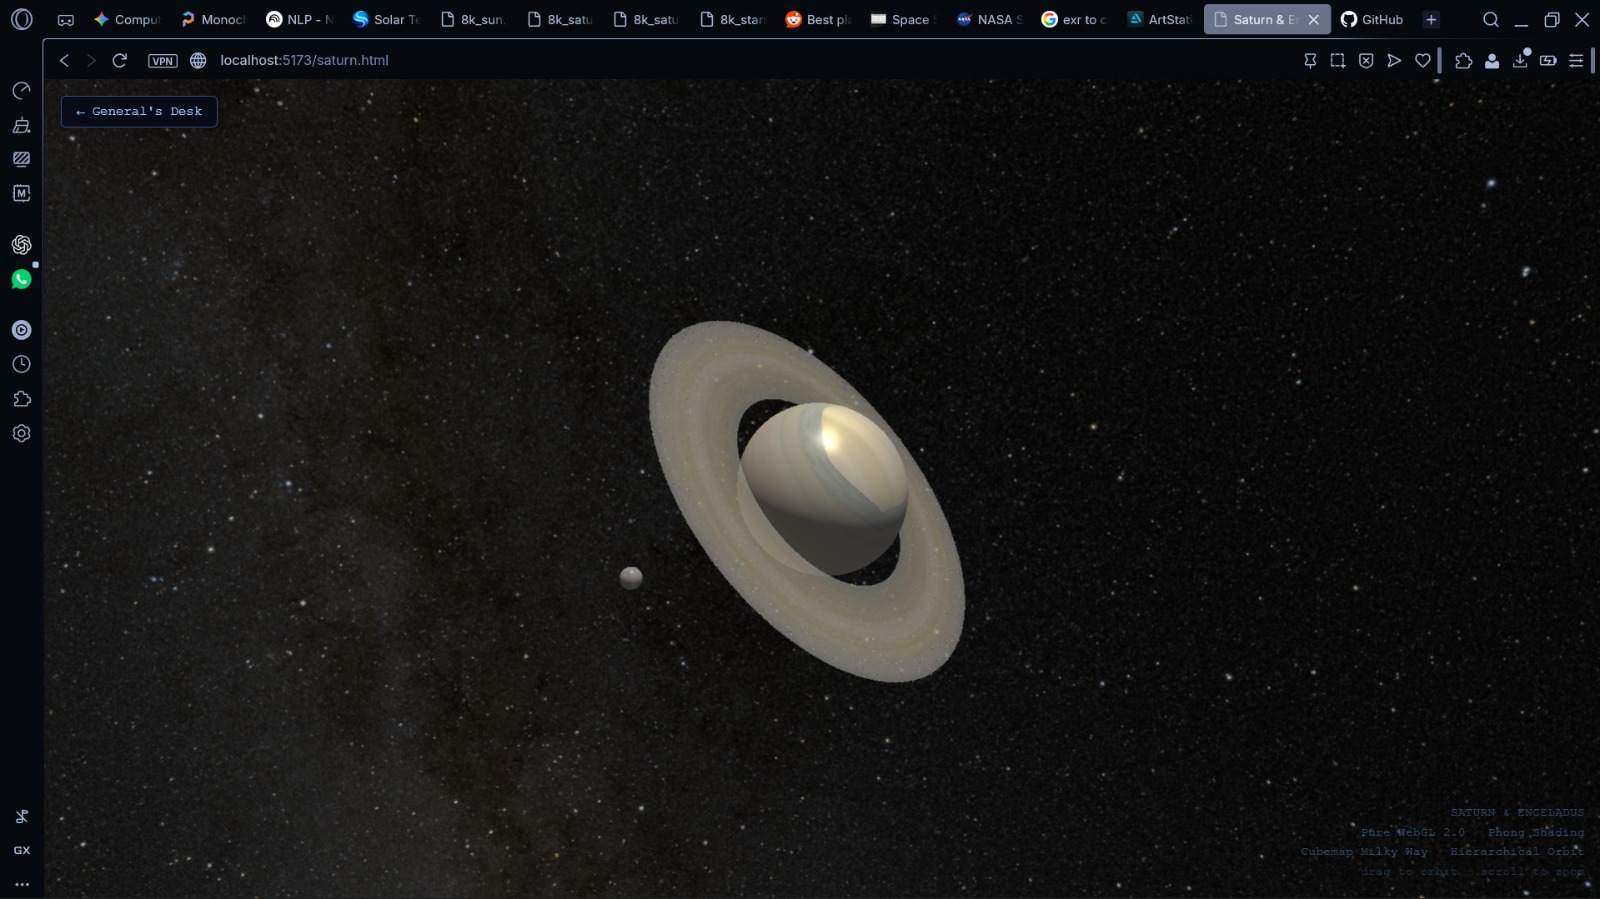
\includegraphics[width=0.56\linewidth]{../Assets/Reference Pictures/Ref2.jpeg}\hfill
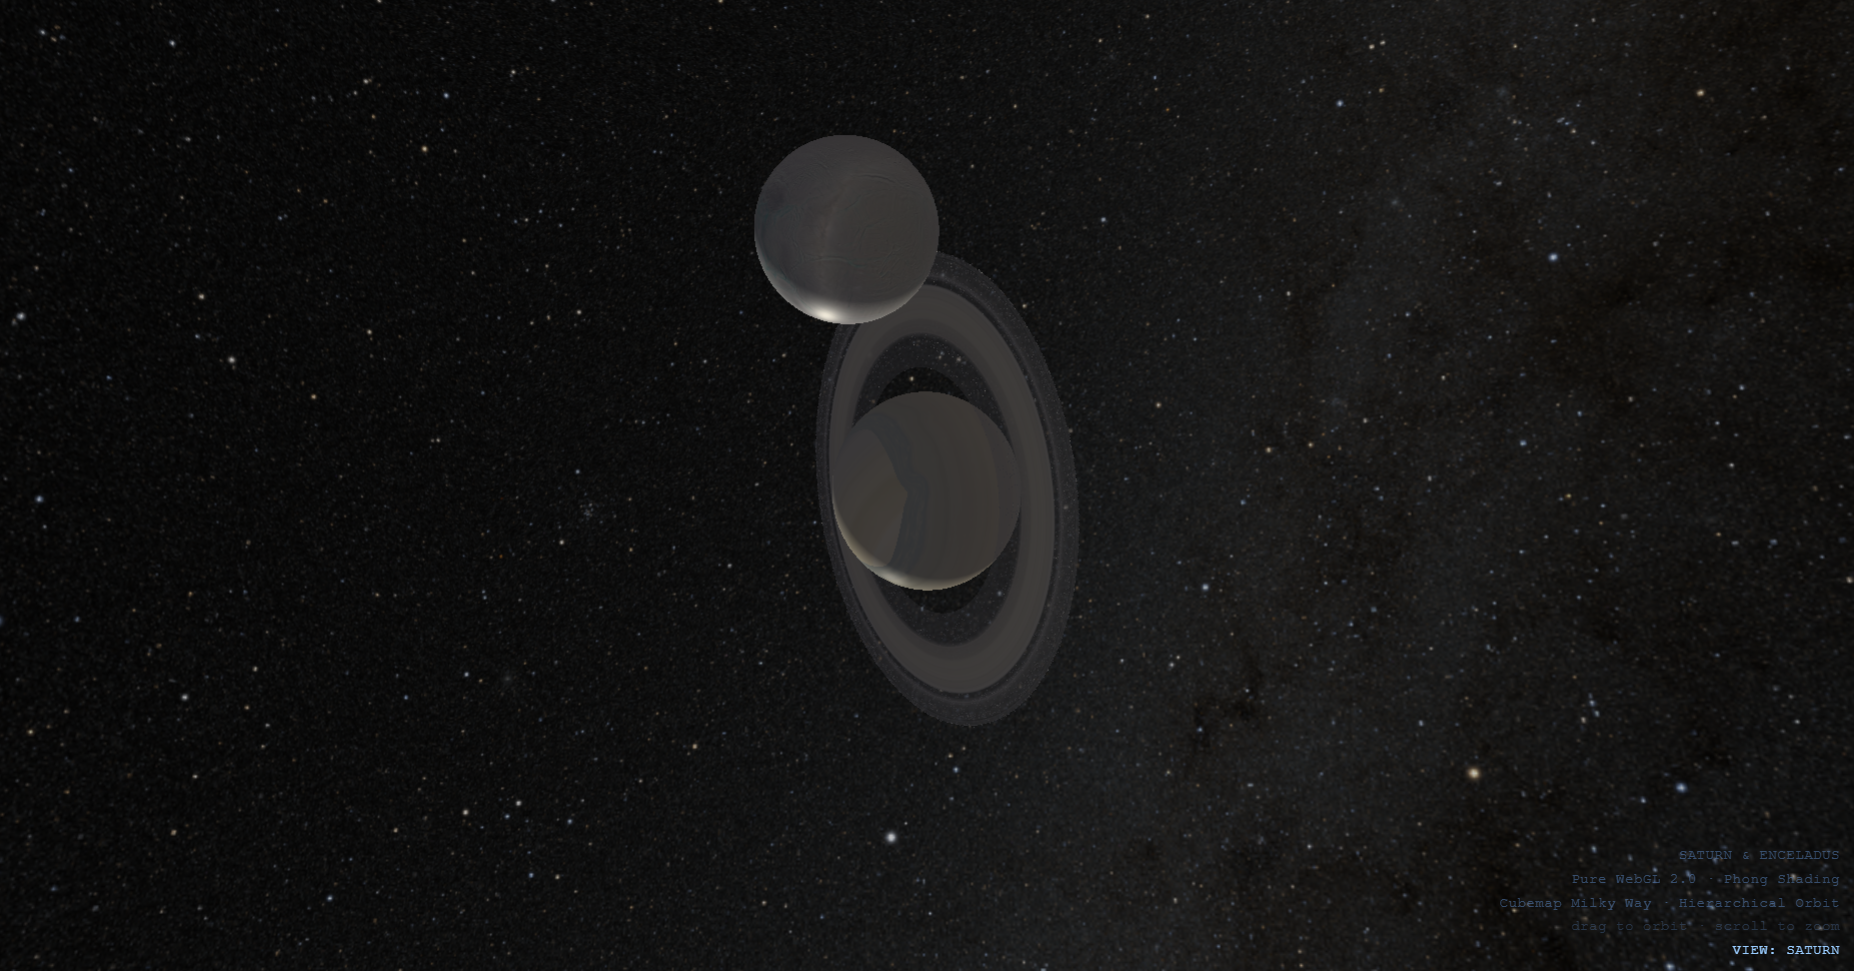
\includegraphics[width=0.41\linewidth]{../Assets/Reference Pictures/Ref1.png}
\\[4pt]
% Row 2
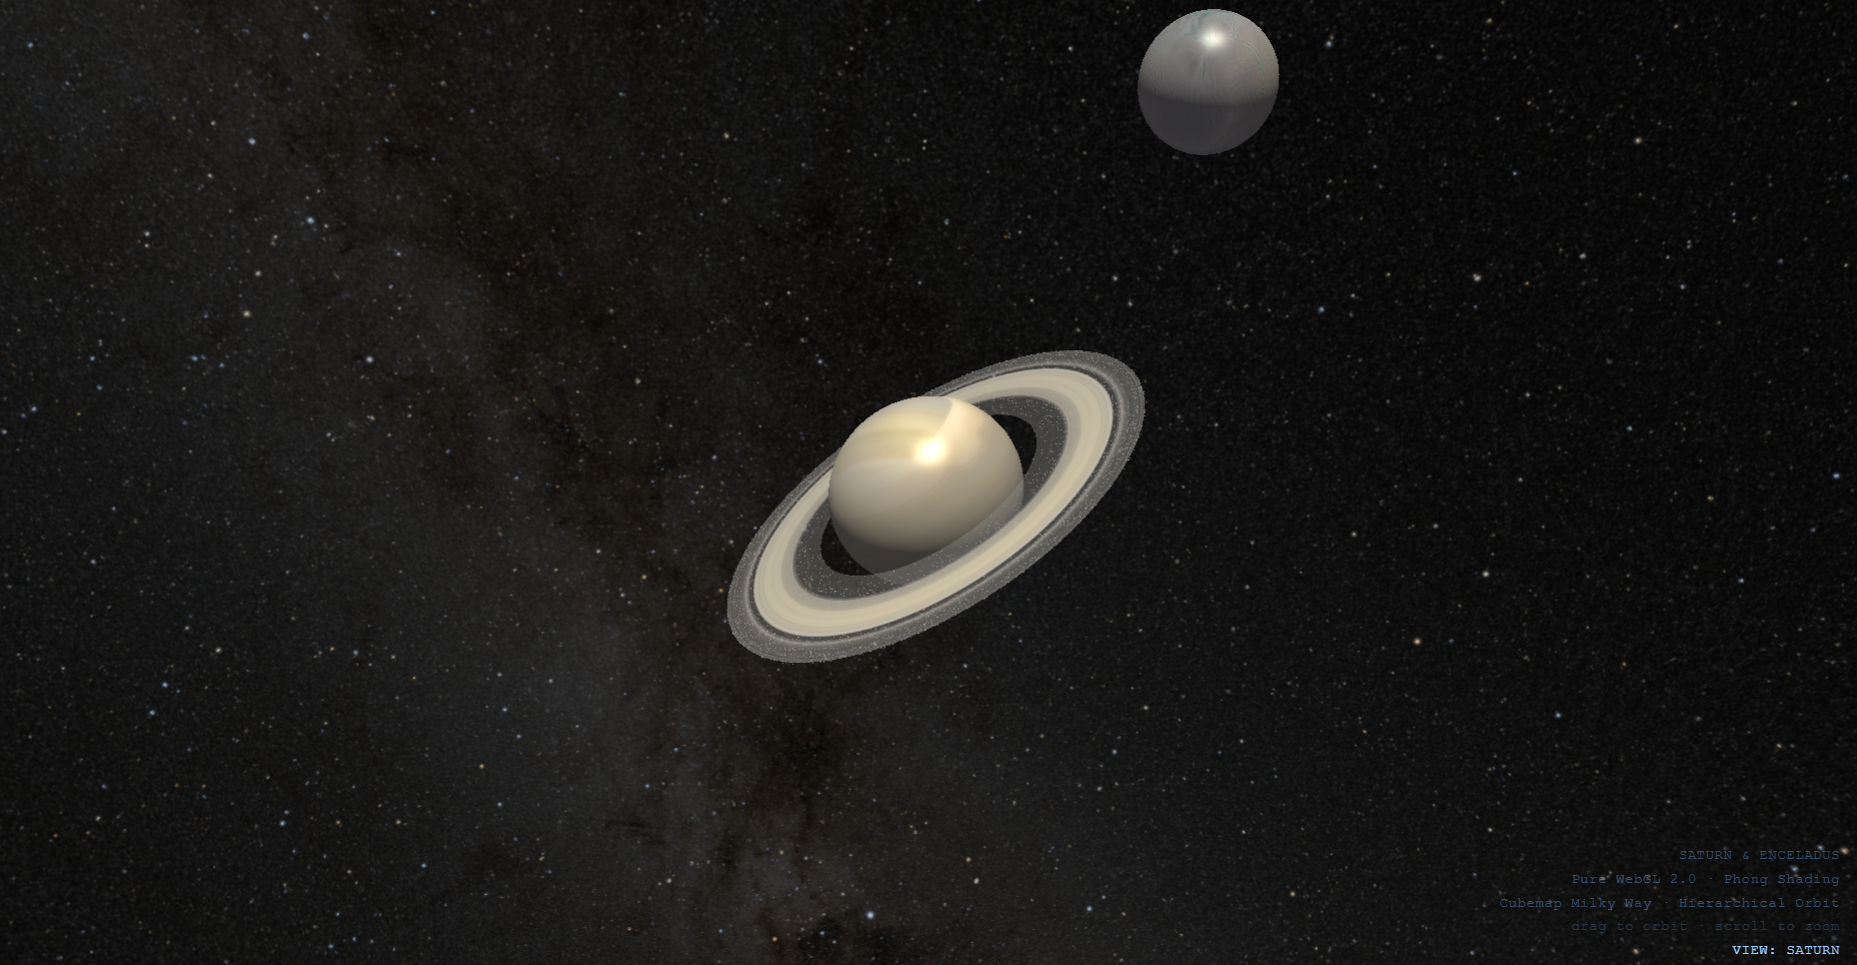
\includegraphics[width=0.48\linewidth]{../Assets/Reference Pictures/Ref3.png}\hfill
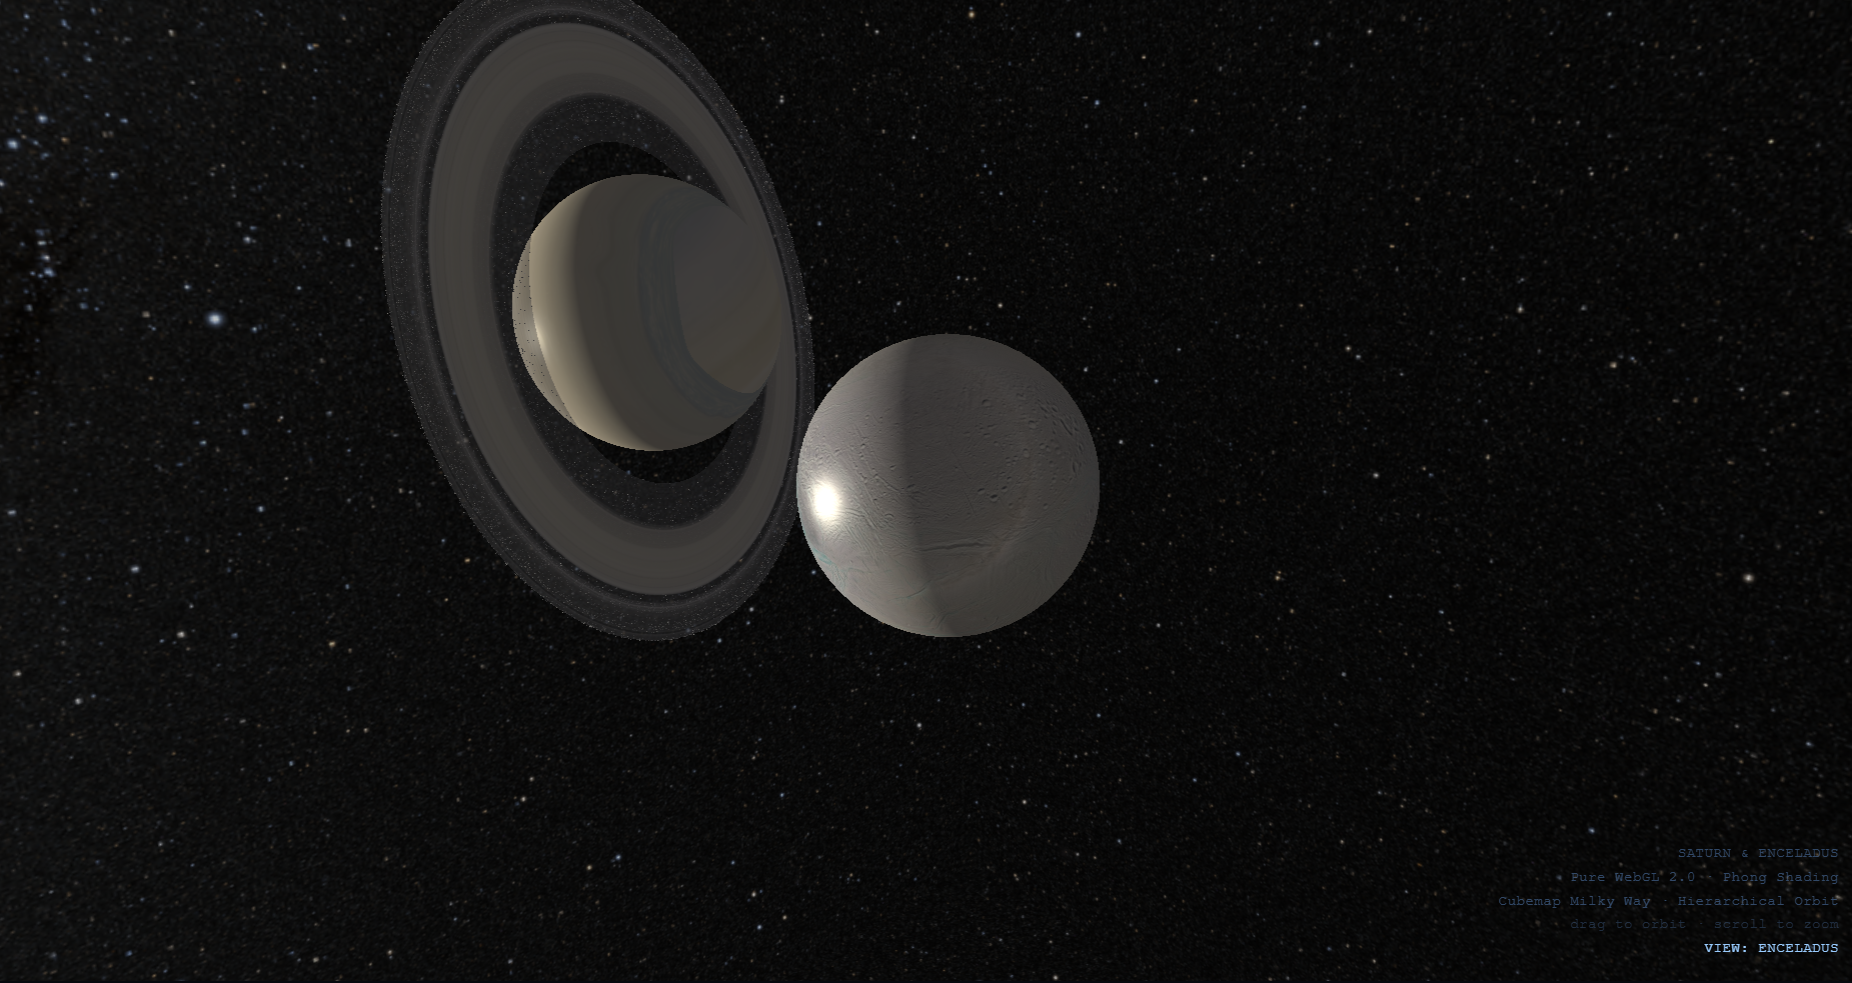
\includegraphics[width=0.48\linewidth]{../Assets/Reference Pictures/Ref4.png}
\\[4pt]
% Row 3
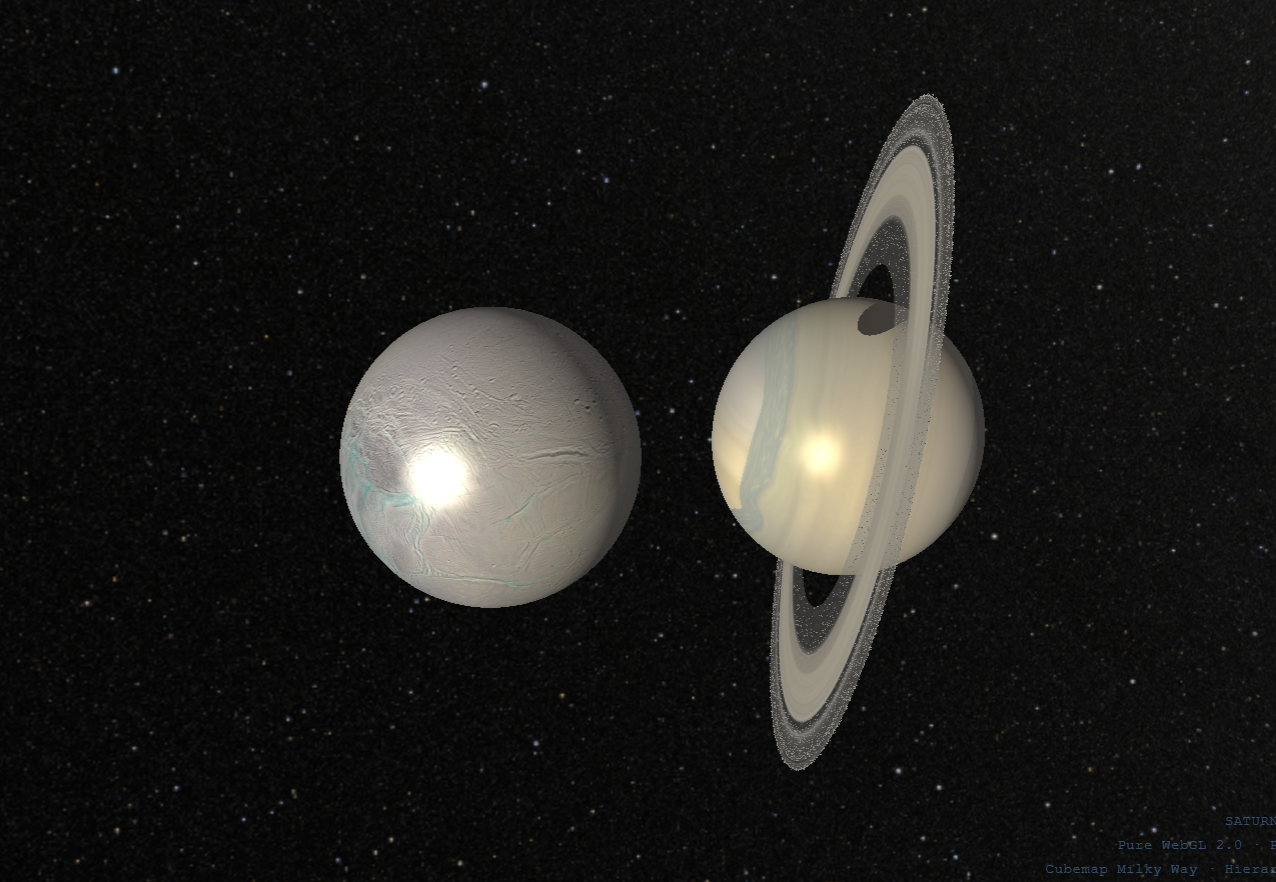
\includegraphics[width=0.70\linewidth]{../Assets/Reference Pictures/Ref5.png}
\\[4pt]
{\small
\textbf{Ref1 (top-right):} Early-stage in-engine render showing Saturn ring
geometry and Enceladus above Saturn against the Milky Way starfield. Captured
during initial shader bring-up. Demonstrates: ring alpha blending, depth
ordering, axial tilt, Phong lighting.

\textbf{Ref2 (top-left):} Full browser screenshot (\texttt{localhost:5173})
with the complete pipeline active --- 8K texture, per-fragment Phong,
Milky Way cubemap skybox, hierarchical orbit, and bloom on Saturn's lit face.
Demonstrates: full pipeline, all advanced techniques combined.

\textbf{Ref3 (mid-left):} Close-up of Saturn + Enceladus showing the Milky
Way environment map reflected on the ring plane. Demonstrates: environment
mapping, bloom post-processing, exponential fog.

\textbf{Ref4 (mid-right):} Enceladus view mode (\texttt{E} key). Enceladus
fills the foreground and its smooth icy surface shows an especially clear
cubemap reflection of the Milky Way starfield, physically consistent with a
high-specular icy moon. Saturn and rings visible in background.
Demonstrates: environment mapping on a high-reflectance surface.

\textbf{Ref5 (bottom):} Both bodies rendered side-by-side showing the
analytical inter-body shadow system. The dark terminator on Enceladus's
facing hemisphere is produced by the ray-sphere occlusion test in the
fragment shader (Saturn blocks the directional sun). Demonstrates:
analytical shadow / occlusion.}
\end{figure}

%──────────────────────────────────────────────────────────────────────────────
\section{Challenges Encountered}

Ring depth ordering was the primary technical hurdle: the alpha-blended ring
plane intersected the planet body and caused z-fighting with incorrect
transparency.
This was resolved by drawing opaque body meshes first (writing to the depth
buffer), then drawing rings with \texttt{depthMask(false)}, blending enabled,
and \texttt{polygonOffset(1,\,1)} to push co-planar fragments back.
The GLB loader had to handle both strided and non-strided \texttt{bufferView}
layouts and two distinct material workflows
(\textit{PBR Metallic-Roughness} and \textit{KHR\_materials\_pbrSpecularGlossiness})
because different asset sources use different GLTF material extensions.
Bloom initially produced halos on non-emissive dark regions because the
brightness threshold was a hard clip; replacing it with a \texttt{smoothstep}
ramp around the threshold eliminated the artefact.
Anisotropic filtering (\texttt{EXT\_texture\_filter\_anisotropic}) must be
queried at runtime as it is not guaranteed across all WebGL~2.0 implementations,
requiring a fallback path.

%──────────────────────────────────────────────────────────────────────────────
\section{Remaining Work}

\begin{itemize}
  \item Verify \texttt{saturn.glb} and \texttt{enceladus.glb} asset pipeline
        through the Vite dev server; confirm GPU memory budget.
  \item Add a loading progress bar tied to the existing XHR
        \texttt{onprogress} callbacks.
  \item Tune Bloom threshold and blur radius for the final submission render.
  \item Improve shadow quality --- current analytical ray-sphere test produces
        a hard binary shadow boundary; replace with a soft penumbra approximation
        (e.g.\ smooth step over the disc edge) for more physically plausible
        eclipse transitions.
  \item Add on-screen HUD: current view mode, orbit angle, camera distance.
  \item Final performance pass --- dirty-flag tracking to reduce per-frame
        uniform uploads.
\end{itemize}

%──────────────────────────────────────────────────────────────────────────────
\section{Scope Adjustments}

No proposed techniques have been removed or replaced.
The set (Bloom 4/5, Environment Mapping 3/5, Fog 2/5, Gamma Correction 2/5)
is intact and fully completed; combined score is $11/10$, satisfying both
requirements ($\geq 6/10$, at least one $\geq 3/5$).
Three un-proposed features were added during implementation:
\textit{analytical inter-body ray-sphere shadows}
(Enceladus eclipsed by Saturn and vice-versa),
\textit{ring alpha blending with correct depth ordering}, and
\textit{anisotropic texture filtering}.
These additions were feasible without scope compromise and improve visual
fidelity without replacing any committed technique.

%──────────────────────────────────────────────────────────────────────────────
\section{External Assets Update}

No assets have been removed since the proposal.
The following were added or confirmed during implementation:

\smallskip
\begin{tabular}{@{}p{4.6cm}p{5.8cm}p{4.4cm}@{}}
\toprule
Asset & Source & Licence \\
\midrule
Saturn 3D model (\texttt{saturn.glb})
  & Sketchfab & CC-BY \\
Enceladus 3D model (\texttt{enceladus.glb})
  & Sketchfab & CC-BY \\
8K Saturn body (\texttt{8k\_saturn.jpg})
  & \href{https://www.solarsystemscope.com/textures/}{solarsystemscope.com}
  & CC-BY \\
Ring alpha mask (\texttt{8k\_saturn\_ring\_alpha.png})
  & \href{https://www.solarsystemscope.com/textures/}{solarsystemscope.com}
  & CC-BY \\
8K Sun texture (\texttt{8k\_sun.jpg})
  & \href{https://www.solarsystemscope.com/textures/}{solarsystemscope.com}
  & CC-BY \\
Milky Way starmap cubemap (6 faces)
  & NASA / STScI --- Gaia DR2 all-sky
  & Public domain \\
\texttt{gl-matrix} v3.4
  & \href{https://npmjs.com/package/gl-matrix}{npmjs.com/package/gl-matrix}
  & MIT \\
\bottomrule
\end{tabular}

\end{document}
